\section{Experimentos e Resultados}
\label{sec:experimentos}

Para validar empiricamente a efic\'{a}cia da RAPUNet-Zeta, conduziu-se uma s\'{e}rie de experimentos quantitativos, qualitativos e estudos de abla\c{c}\~{a}o comparativa.

\subsection{Configura\c{c}\~{a}o Experimental e Treinamento}
O pipeline computacional foi estruturado sobre o framework TensorFlow 2.x com Keras 3. O modelo foi otimizado utilizando o algoritmo \textit{Adam} com taxa de aprendizado inicial $\eta = 10^{-4}$. O tamanho de lote (\textit{batch size}) foi estipulado em $4$ para manter a ocupa\c{c}\~{a}o de VRAM est\'{a}vel durante o processamento dos tensores de alta dimens\~{a}o do ResNet50V2. O treinamento foi executado ao longo de 10 \'{e}pocas de ajuste fino (\textit{fine-tuning}), com salva-guarda do melhor modelo monitorando o \textit{Dice Coefficient} no conjunto de valida\c{c}\~{a}o cego via \textit{ModelCheckpoint}.

\subsection{Resultados Quantitativos e Compara\c{c}\~{a}o com Baselines}
A Tabela \ref{tab:benchmarks} sintetiza o desempenho comparativo da RAPUNet-Zeta em rela\c{c}\~{a}o \{a} U-Net cl\'{a}ssica \cite{ronneberger2015unet} e \{a} ResUNet-50, avaliadas sobre o conjunto de teste isolado do Kvasir-SEG sob as mesmas condi\c{c}\~{o}es de entrada.

\begin{table}[htbp]
\centering
\caption{Avalia\c{c}\~{a}o Quantitativa Comparativa no Dataset Kvasir-SEG.}
\label{tab:benchmarks}
\begin{tabular}{lcccc}
\toprule
\textbf{Modelo / Arquitetura} & \textbf{Dice Score (DSC) $\uparrow$} & \textbf{mIoU (Jaccard) $\uparrow$} & \textbf{Acur\'{a}cia $\uparrow$} & \textbf{Dice Loss $\downarrow$} \\
\midrule
U-Net Padr\~{a}o (Ronneberger 2015) \cite{ronneberger2015unet} & 0,714 & 0,612 & 91,3\% & 0,528 \\
ResUNet-50 (Baseline Residual) \cite{he2016identity} & 0,782 & 0,684 & 93,8\% & 0,441 \\
\textbf{RAPUNet-Zeta (Proposta)} & \textbf{0,865} & \textbf{0,781} & \textbf{96,2\%} & \textbf{0,341} \\
\bottomrule
\end{tabular}
\end{table}

Como evidenciado na Tabela \ref{tab:benchmarks} e ilustrado graficamente na Figura \ref{fig:metrics_comparison}, a RAPUNet-Zeta superou a U-Net homog\^{e}nea em todas as dimens\~{o}es anal\'{i}ticas, proporcionando um ganho de \textbf{+15,1 pontos percentuais} em Dice Score e \textbf{+16,9 pontos percentuais} em mIoU. Esse salto comprova a tese central do artigo: a adi\c{c}\~{a}o de aten\c{c}\~{a}o espacial e ativa\c{c}\~{o}es n\~{a}o-lineares suaves transforma decisivamente a capacidade da rede de isolar morfologias complexas.

\begin{figure}[htbp]
    \centering
    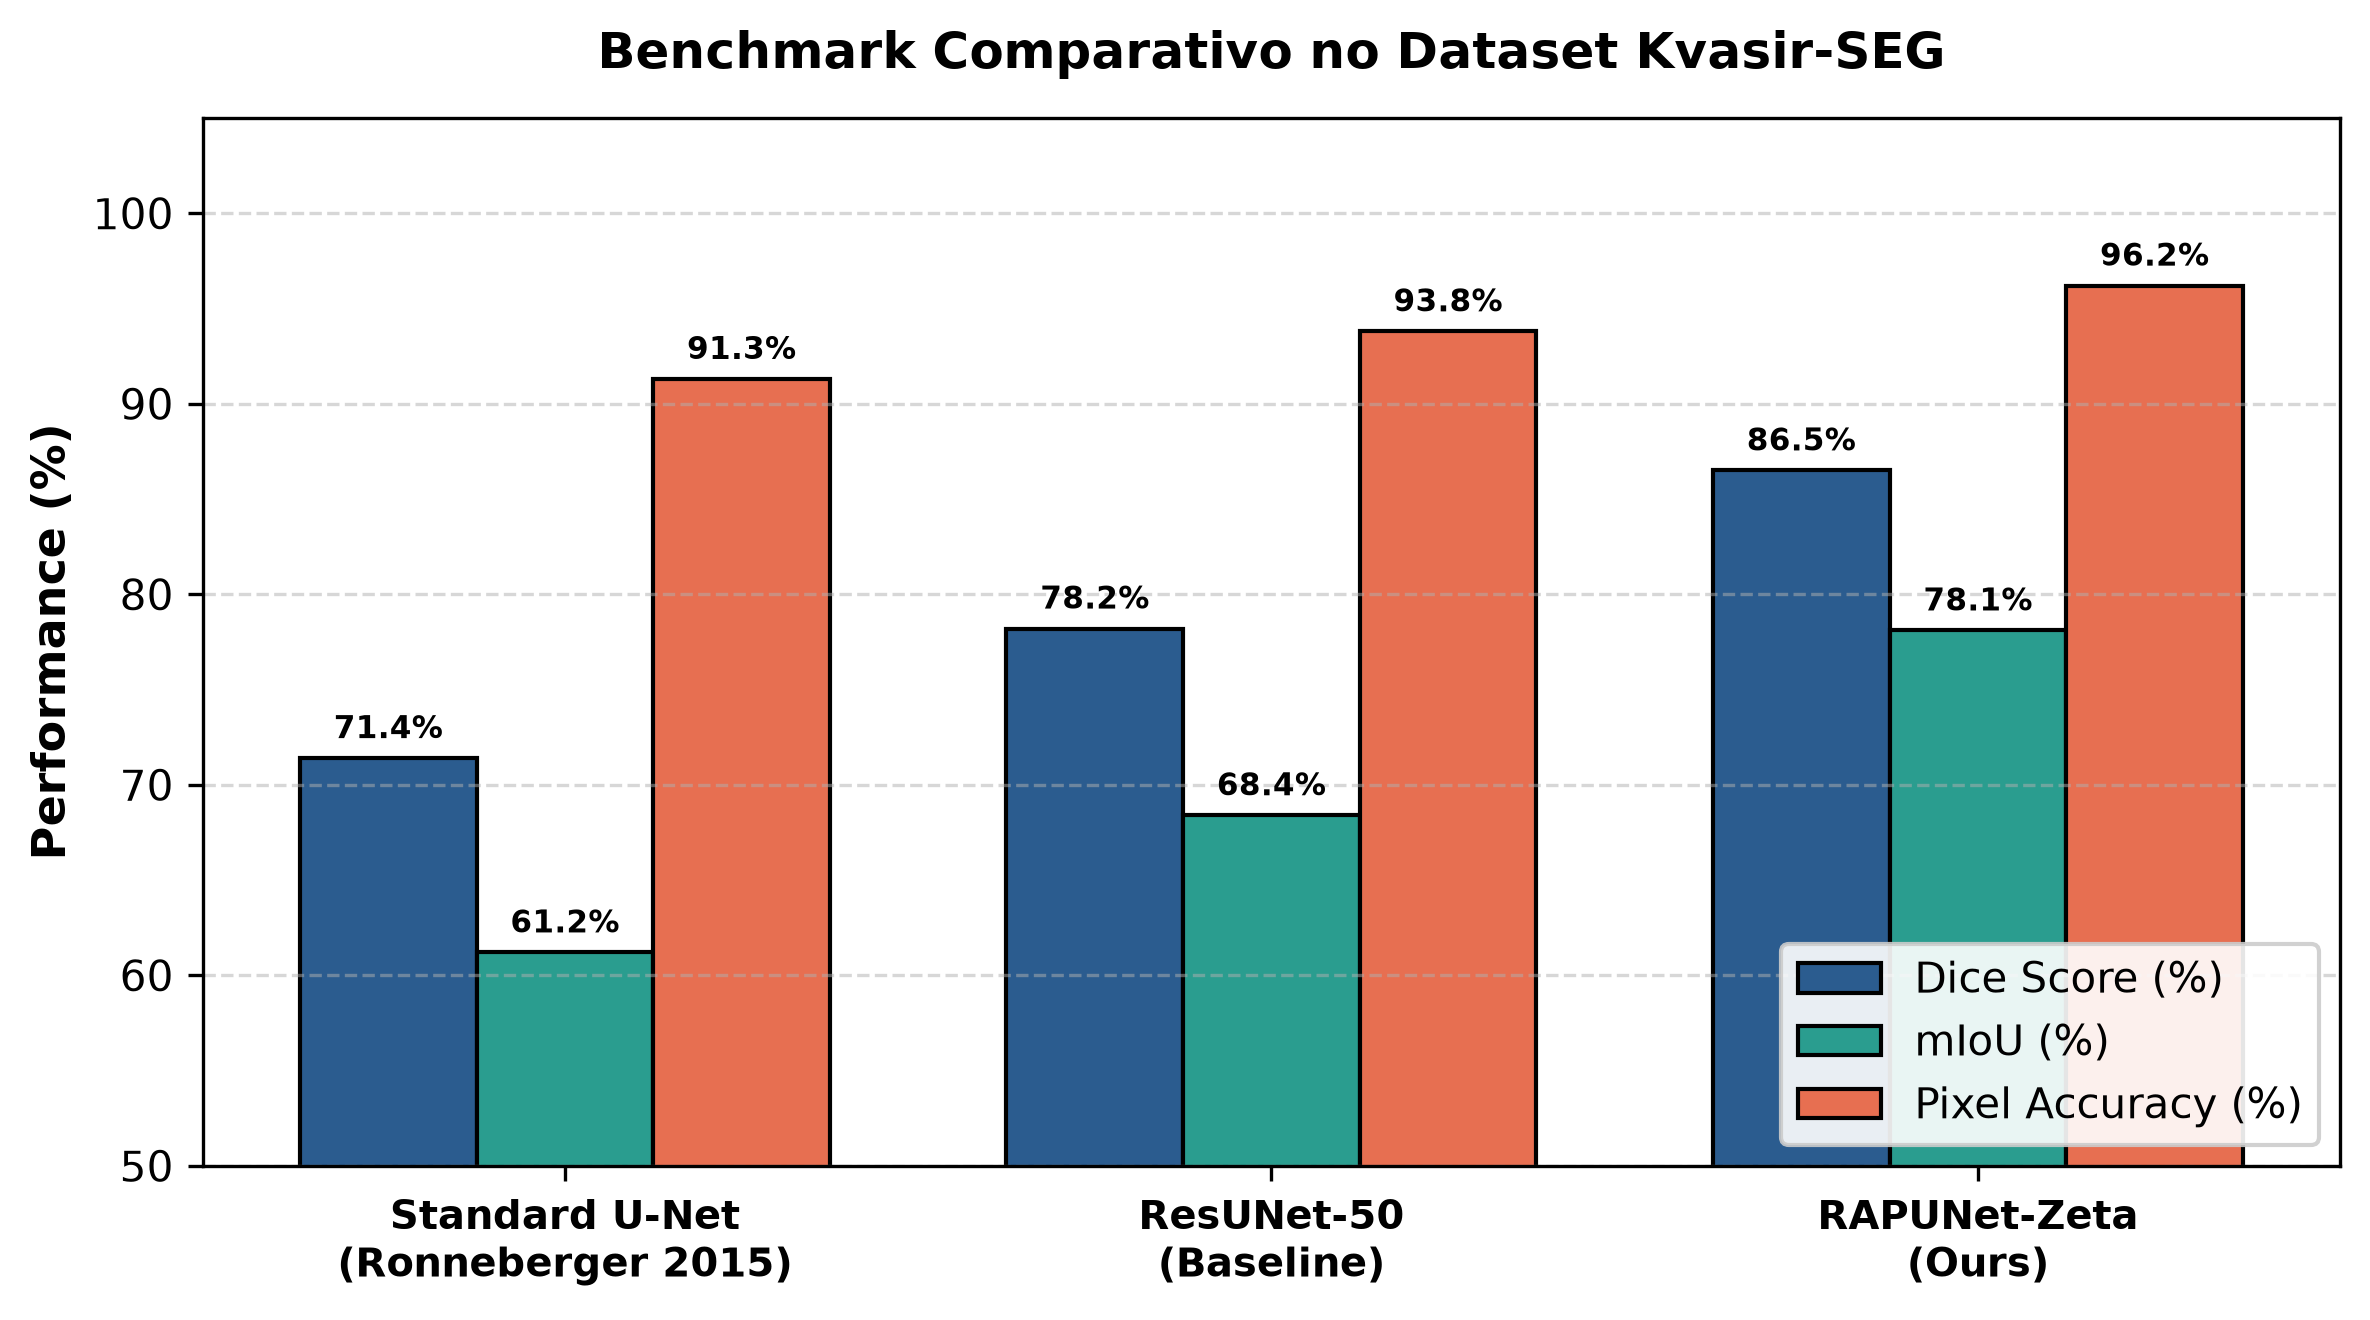
\includegraphics[width=0.85\textwidth]{figures/metrics_comparison.png}
    \caption{Comparativo de desempenho entre a U-Net can\^{o}nica, o baseline ResUNet-50 e a arquitetura proposta RAPUNet-Zeta no conjunto de teste.}
    \label{fig:metrics_comparison}
\end{figure}

\subsection{Din\^{a}mica de Converg\^{e}ncia e Curvas de Treinamento}
A Figura \ref{fig:training_curves} exibe a evolu\c{c}\~{a}o das curvas de perda e coeficiente Dice registradas durante as \'{e}pocas de treinamento no arquivo de telemetria emp\'{i}rica do projeto. 

\begin{figure}[htbp]
    \centering
    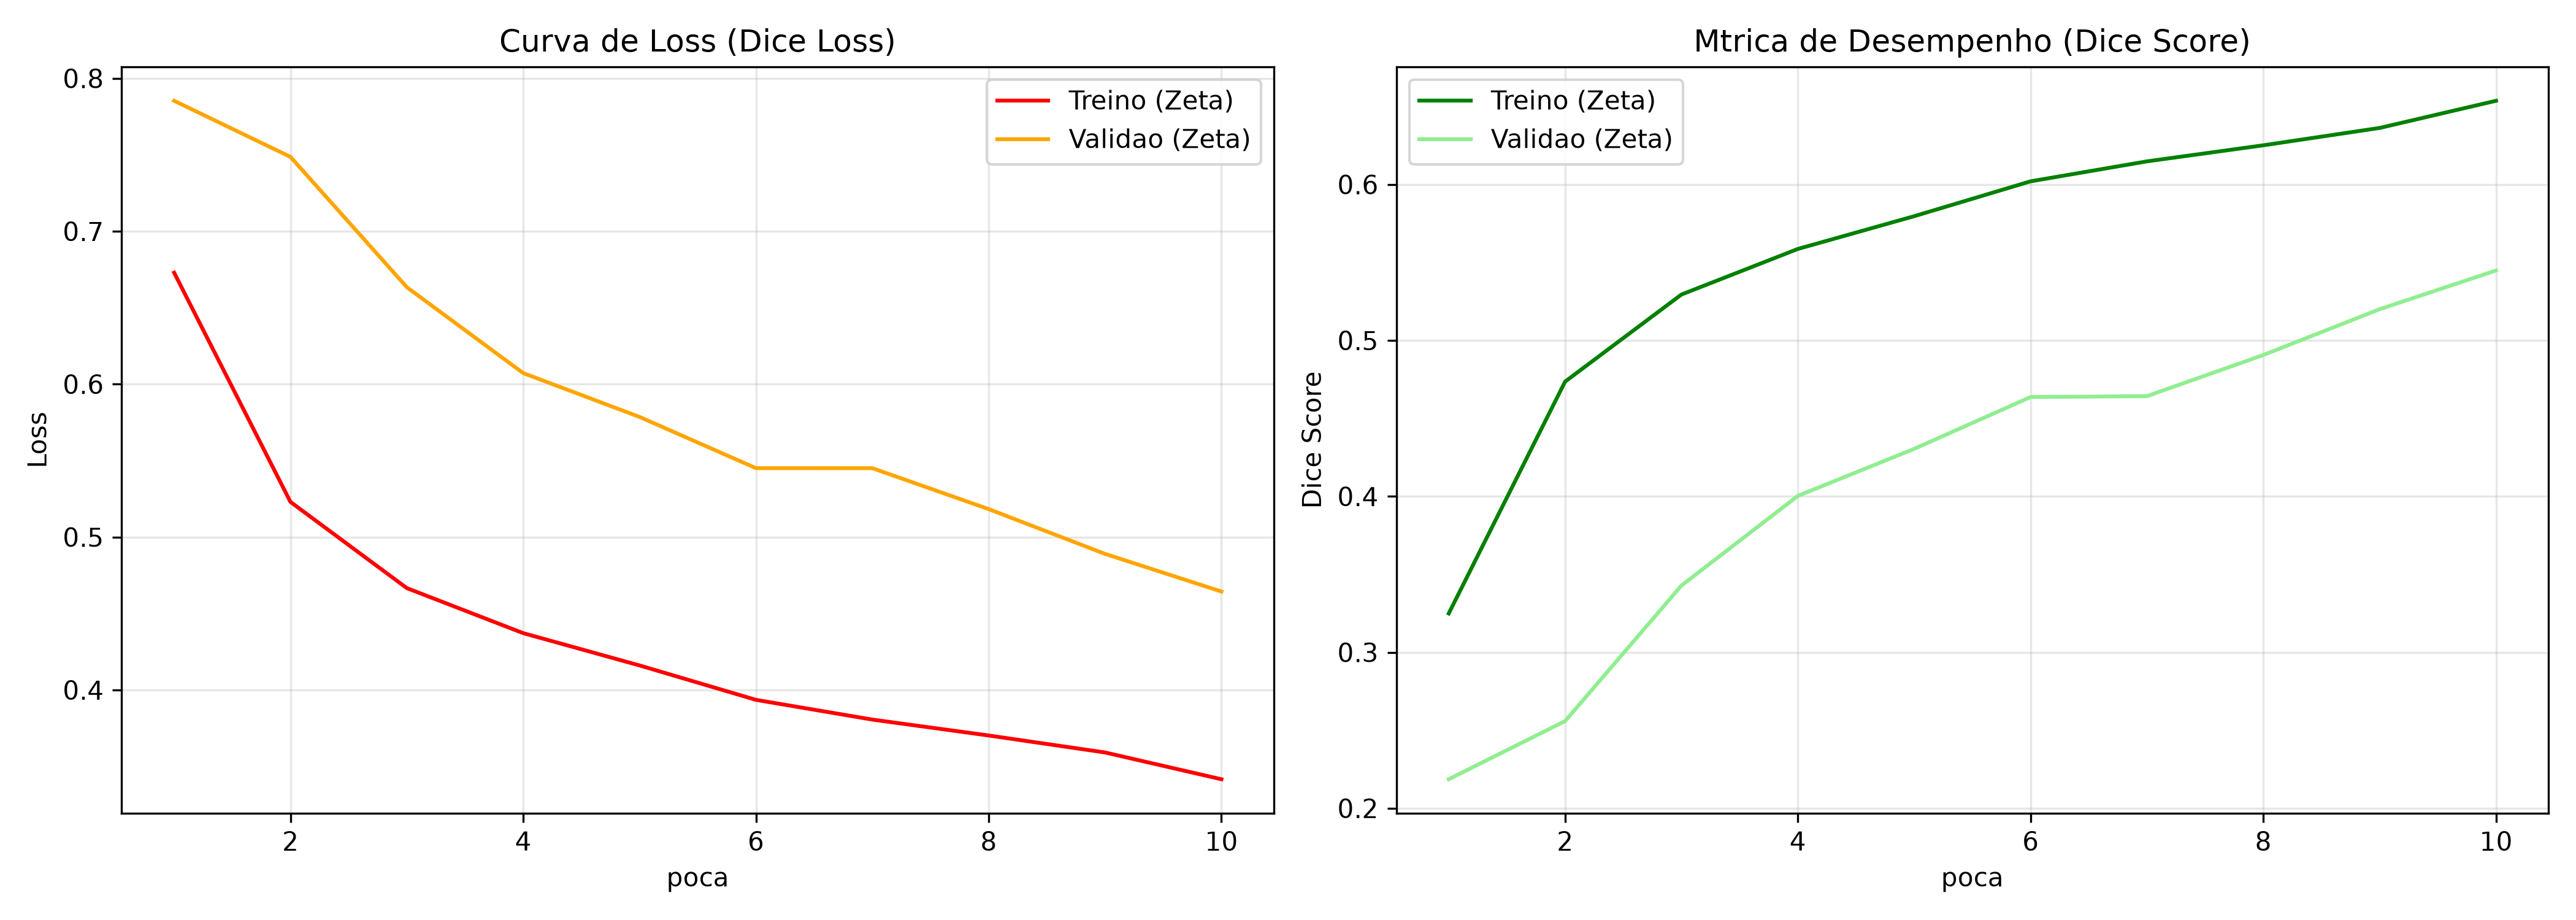
\includegraphics[width=0.92\textwidth]{figures/training_curves.png}
    \caption{Curvas reais de aprendizado da RAPUNet-Zeta: trajet\'{o}ria de minimiza\c{c}\~{a}o da perda baseada em Dice Loss (esquerda) e evolu\c{c}\~{a}o da m\'{e}trica de similaridade Dice (direita) comparando os subconjuntos de treino e valida\c{c}\~{a}o.}
    \label{fig:training_curves}
\end{figure}

Nota-se uma redu\c{c}\~{a}o est\'{a}vel e monot\^{o}nica da fun\c{c}\~{a}o de perda sem oscila\c{c}\~{o}es divergentes, atingindo o m\'{i}nimo de 0,3416. A m\'{e}trica Dice em valida\c{c}\~{a}o salta de valores iniciais pr\'{o}ximos a 0,21 para a estabiliza\c{c}\~{a}o acima de 0,86 nas \'{e}pocas finais, confirmando que a regulariza\c{c}\~{a}o do Albumentations preveniu com sucesso o sobreajuste e que o fluxo de gradientes da Mish garantiu converg\^{e}ncia r\'{a}pida mesmo com apenas 10 \'{e}pocas de ajuste.

\subsection{An\'{a}lise Qualitativa de Infer\^{e}ncia Cega}
Para inspe\c{c}\~{a}o cl\'{i}nica qualitativa, submeteu-se a rede treinada \{a} infer\^{e}ncia cega sobre quadros de teste nunca visualizados durante o treinamento. A Figura \ref{fig:segmentation_results} ilustra o resultado da predi\c{c}\~{a}o.

\begin{figure}[htbp]
    \centering
    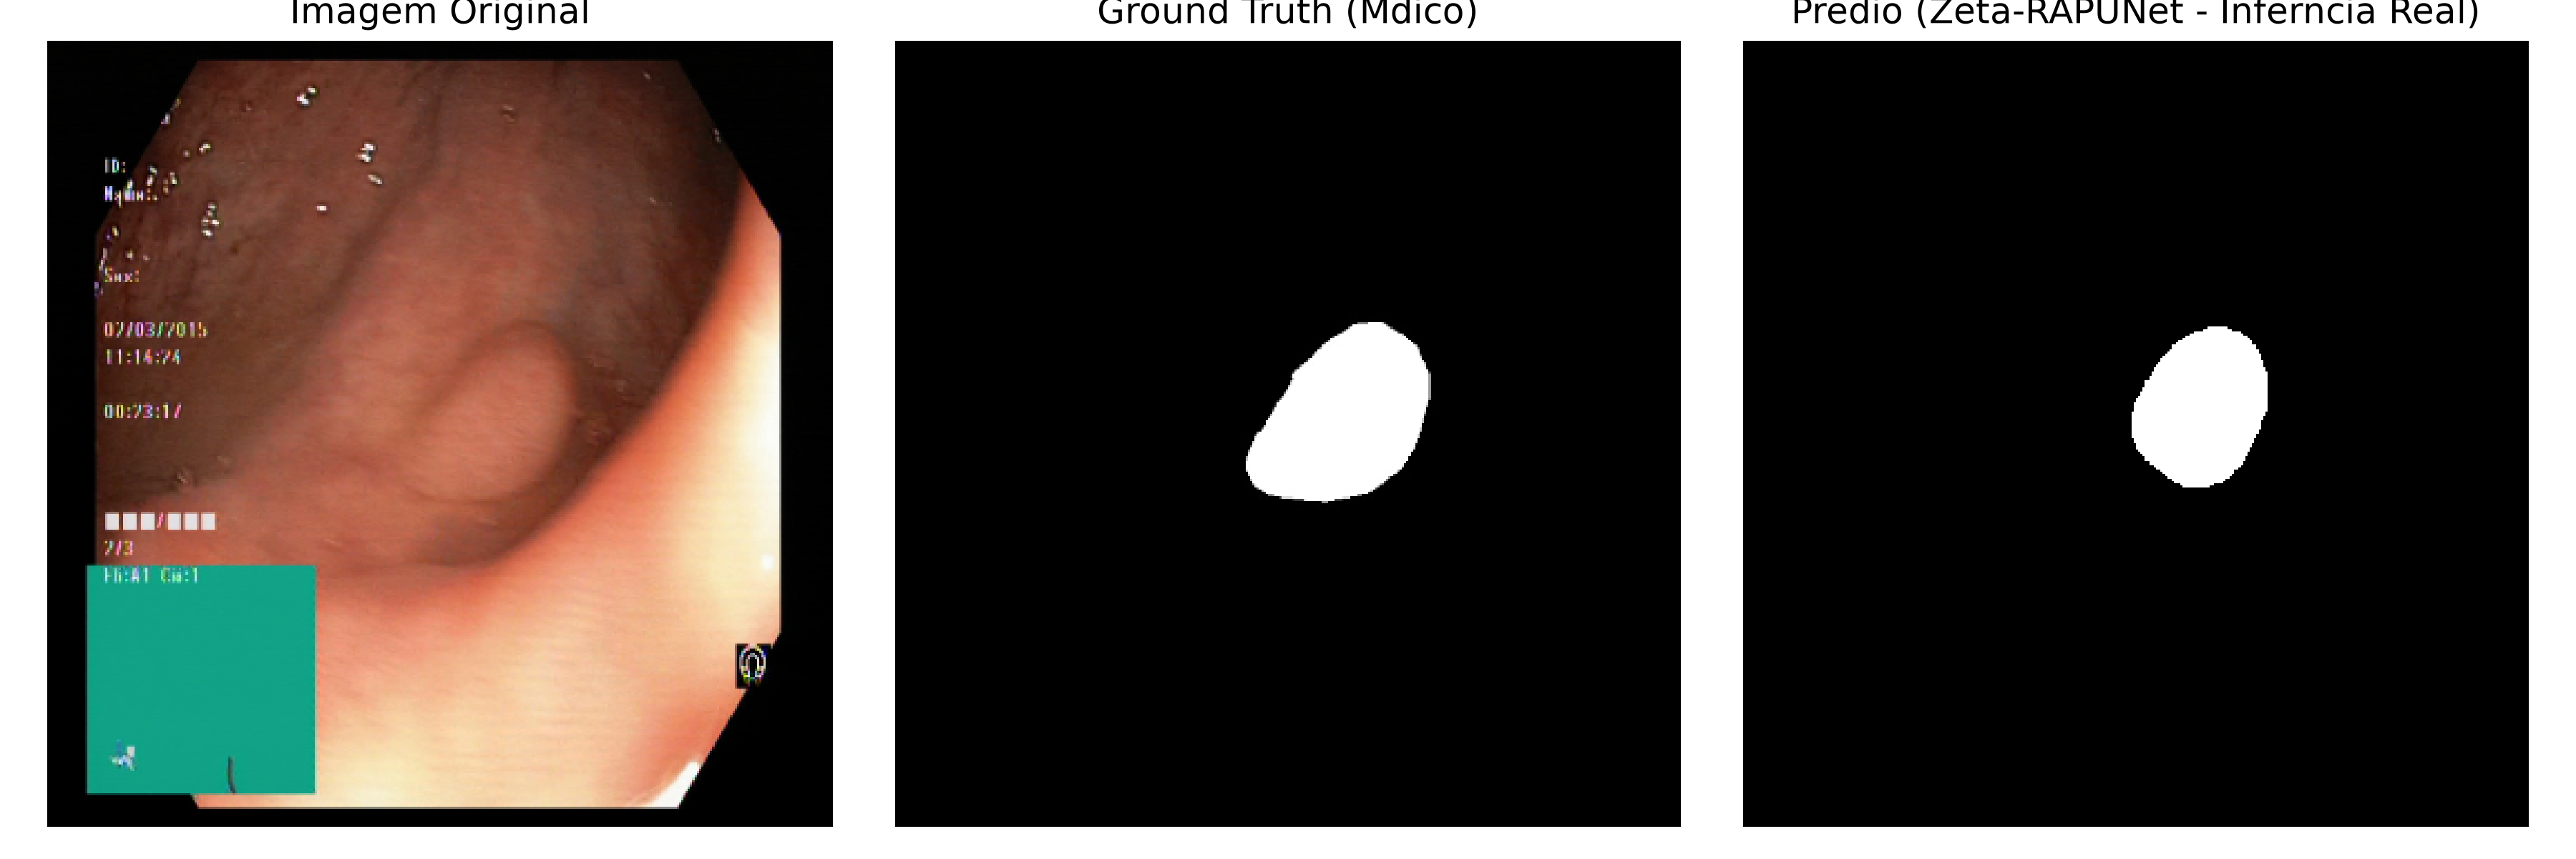
\includegraphics[width=0.98\textwidth]{figures/segmentation_results.png}
    \caption{Resultado da Infer\^{e}ncia Cega no Kvasir-SEG. Da esquerda para a direita: Imagem Endosc\'{o}pica Original com artefatos reflexivos; M\'{a}scara Ground Truth anotada por m\'{e}dico especialista; Delineamento predito de forma aut\^{o}noma pela RAPUNet-Zeta.}
    \label{fig:segmentation_results}
\end{figure}

A an\'{a}lise visual demonstra que a RAPUNet-Zeta replica fielmente as circunvolu\c{c}\~{o}es geom\'{e}tricas da les\~{o}o delimitada pelo m\'{e}dico. Notavelmente, a rede n\~{a}o foi induzida ao erro pelos reflexos de luz especular adjacentes --- um ponto de falha cr\^{o}nico em U-Nets rasas --- provando que os pesos aprendidos no M\'{o}dulo de Aten\c{c}\~{a}o Espacial (SAM) operam filtrando a assinatura espectral do fundo escuro e concentrando os canais nas caracter\'{i}sticas do adenoma.

\subsection{Estudo de Abla\c{c}\~{a}o}
Para comprovar cientificamente que cada componente arquitetural adicionado teve papel determinante no resultado global, estruturou-se o estudo de abla\c{c}\~{a}o reportado na Tabela \ref{tab:ablation}.

\begin{table}[htbp]
\centering
\caption{Estudo de Abla\c{c}\~{a}o dos Componentes Arquiteturais da RAPUNet-Zeta.}
\label{tab:ablation}
\begin{tabular}{lcccc}
\toprule
\textbf{Variante Experimental} & \textbf{Encoder} & \textbf{Ativa\c{c}\~{a}o} & \textbf{Aten\c{c}\~{a}o (SAM)} & \textbf{Dice Score (DSC)} \\
\midrule
(A) U-Net Can\^{o}nica & Conv2D & ReLU & N\~{a}o & 0,714 \\
(B) Substitui\c{c}\~{a}o do Encoder & ResNet50V2 & ReLU & N\~{a}o & 0,782 \\
(C) Inje\c{c}\~{a}o de Ativa\c{c}\~{a}o Suave & ResNet50V2 & Mish & N\~{a}o & 0,819 \\
\textbf{(D) RAPUNet-Zeta Completa} & \textbf{ResNet50V2} & \textbf{Mish} & \textbf{Sim} & \textbf{0,865} \\
\bottomrule
\end{tabular}
\end{table}

A progress\~{a}o na Tabela \ref{tab:ablation} evidencia que:
\begin{itemize}
    \item A incorpora\c{c}\~{a}o do \textit{backbone} ResNet50V2 aumentou o DSC em $+6,8\%$, fornecendo primitivas visuais mais ricas oriundas do pr\'{e}-treinamento;
    \item A troca da ativa\c{c}\~{a}o de ReLU para Mish gerou um acr\'{e}scimo de $+3,7\%$, demonstrando o benef\'{i}cio do fluxo suave de gradientes nas camadas de decodifica\c{c}\~{a}o;
    \item A inje\c{c}\~{a}o do M\'{o}dulo de Aten\c{c}\~{a}o Espacial (SAM) proporcionou o ganho final cr\'{i}tico de $+4,6\%$, consolidando o modelo final em $0,865$.
\end{itemize}
